\chapter{GRASS}\label{sec:grass}\index{GRASS}
The GRASS plugin adds the following features to QGIS:
\begin{compactitem}
\item Add GRASS vector layers
\item Add GRASS raster layers
\item Vector layers digitizing
\item Changing of the GRASS region
\end{compactitem}
\section{Starting QGIS with
GRASS}\label{sec:starting_grass}\index{GRASS!starting QGIS}
When using the GRASS plugin, QGIS can be started in two ways: from the GRASS shell or from a regular shell.
\subsection{From GRASS shell}

If QGIS is started from the GRASS shell (GRASS started by grass57 command), no
additional settings are required. \index{GRASS!shell}
\subsection{Outside GRASS shell}

If QGIS is not started from the GRASS shell, the environment variables must be properly set before starting QGIS.
 
The path to GRASS libraries must be added to LD\_LIBRARY\_PATH environment
variable. For example (in bash): \index{GRASS!environment settings}
\begin{verbatim}
    export LD_LIBRARY_PATH=/usr1/grass57/dist.i686-pc-linux-gnu/lib:$LD_LIBRARY_PATH
\end{verbatim}    
 
The GISBASE environment variable must be set to the full path of the directory where GRASS is installed (the same as used for --with-grass= option). For example (in bash):
\begin{verbatim}
    export GISBASE=/usr1/grass57/dist.i686-pc-linux-gnu 
\end{verbatim}
\section{Loading GRASS Data}\index{GRASS!loading data}
With the GRASS plugin loaded, you can load a vector or raster layer using the appropriate button on the toolbar. \begin{Tip}\caption{\textsc{GRASS Data Loading}}
\qgistip{If you have problems loading data or QGIS terminates abnormally, check to make sure you have started GRASS properly as described in Section \ref{sec:starting_grass}.
}
\end{Tip} 
\section{Vector Data Model}\index{GRASS!vector data model}
It is important to understand the GRASS vector data model prior to
digitizing.\index{GRASS!digitizing}
In general, GRASS uses a topological vector model.\index{GRASS!topology} This
means that areas are not represented as closed polygons, but by one or more
boundaries. A boundary between two adjacent areas is digitized only once, and it
is shared by both areas. Boundaries must be connected without gaps. An area is
identified (labeled) by the centroid of the area.

Besides boundaries and centroids, a vector map can also contain
points and lines. All these geometry elements can be mixed
in one vector.

It is possible to store more 'layers' in one vector dataset. For example,
fields, forests and lakes can be stored in one vector. Adjacent
forest and lake can share the same boundary, but they have separate attribute tables.
It is also possible to attach attributes to boundaries. For example, the boundary between lake and forest is a road with different attribute table.
%In addition, one geometry element can represent a geometry for more
%features. For example, a road can be a marked turistic route at the same 
%time.

The 'layer' of the feature is defined by 'field' (sorry for this name).
'Field' is the number which defines if the geometry is forest or lake.
For now, it can be only a number, in the future GRASS will also support  
names as fields in the user interface.

Attributes are stored in external database tables, for example
DBF, PostgreSQL, etc.\index{GRASS!attribute storage}

Attributes in database tables are linked to geometry elements
using 'category'.\index{GRASS!attribute linkage} 'Category' (key, ID) is an
integer attached to geometry primitives, and it is used as the link to one
column in the database table.
\begin{Tip}\caption{\textsc{Learning the GRASS Vector Model}}
\qgistip{The best way to learn the GRASS vector model and its capabilities
is to download the demo mapset from \url{http://mpa.itc.it/radim/g51/g51test-12-multi.tar.gz}.
Extract the mapset, add all layers from vector 'multi' to QGIS, and query attributes.
Finaly start editing of vector 'multi', to see how those layers are stored.
}
\end{Tip} 
\section{Digitizing and Editing Tools}\index{GRASS!digitizing tools}
\label{grass_digitising}
The digitizing tools for GRASS vector layers are accessed using the \textsl{Edit GRASS Vector Layer} tool on the toolbar. Make sure you have loaded a GRASS vector and it is the selected layer in the legend before clicking on the edit tool. In this release, the vector must exist prior to beginning to edit. The ability to create a new "empty" layer will be added in a future version. Figure \ref{fig:grass_edit} shows the GRASS Edit dialog that is displayed when you click on the edit tool. 
\begin{figure}[h]
   \begin{center}
   \caption{GRASS Edit Dialog}\label{fig:grass_edit}\smallskip
   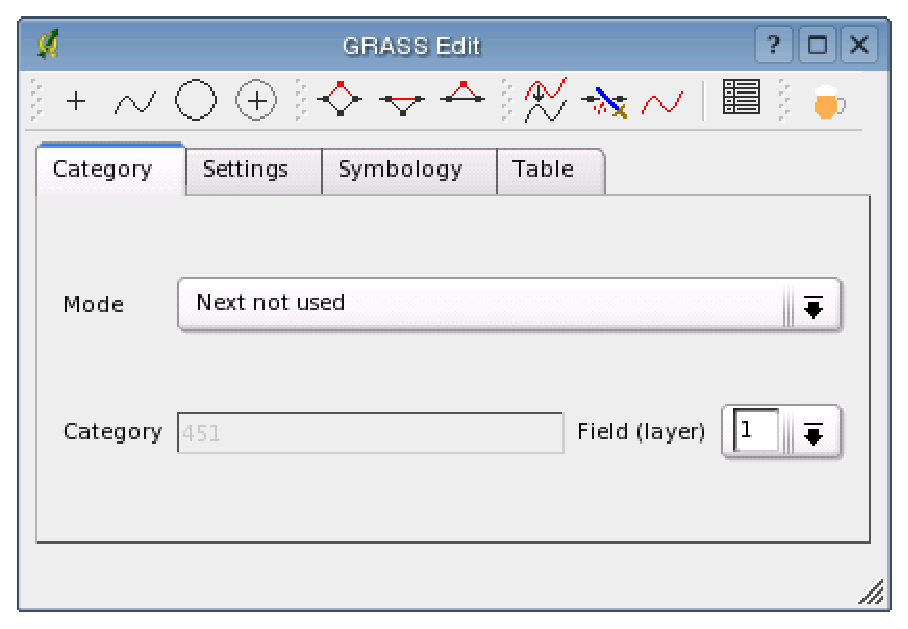
\includegraphics[scale=.7]{qgis_user_guide_images/grassedit}
\end{center}  
\end{figure}
The tools and settings are discussed in the following sections.
\subsection{Toolbar}
Table \ref{tab:grass_tools} lists the digitizing tools provided by the GRASS plugin. These correspond to the tool buttons in the toolbar(s) across the top of the dialog.
\begin{table}[h]\index{GRASS!digitizing tools}

\centering
\caption{GRASS Digitizing Tools}\label{tab:grass_tools}\medskip
 \begin{tabular}{|l|p{5in}|}
 \hline \textbf{Tool} & \textbf{Purpose} \\
\hline New Point & digitize new point \\
\hline New Line &  digitize new line (finish by selecting new tool) \\
\hline New Boundary & digitize new boundary (finish by selecting new tool)\\
\hline New Centroid & digitize new centroid (label existing area)\\
\hline Move vertex & select one vertex of existing line or boundary and identify new position\\
\hline Add vertex & add a new vertex to existing line\\
\hline Delete vertex & delete one vertex from existing line (confirm selected vertex by another click)\\
\hline Move line & select existing line and click on new position\\
\hline Split line & split an existing line to 2 parts\\
\hline Delete line & delete existing line (confirm selected line by another click)\\
\hline Edit attributes & edit attributes of existing element (note that one element can represent more features, see above)\\
\hline Mug & close digitizing session\\
\hline
\end{tabular}
\end{table}
\subsection{Category Tab}\index{GRASS!category settings}
This tab allows you to set the way in which the category will be assigned to each new feature and/or assign a category to a feature.
\begin{compactitem}
\item Mode: what category should be attached to geometry
\begin{compactitem}
\item Next not used - next category not yet used in vector
\item Manual entry - define the category in 'Category entry'
\item No category - digitize geometry without category
\end{compactitem}
\item Category - a number (ID) attached to digitized feature
\item Field - feature (attribute table) identification
\end{compactitem}
\subsection{Settings Tab} \index{GRASS!snapping tolerance}
This tab allow you to set the snapping in screen pixels. This is the threshold in pixels in which new points or line ends are snapped to existing nodes. This helps prevent gaps or dangles between boundaries

\subsection{Symbology Tab}\index{GRASS!symbology settings}
This tab allows you to view and set symbology for various geometry types and their topological status (e.g. closed / opened boundary).

\subsection{Table} \index{GRASS!table editing}
This tab provides the means to view, create, or modify the database table for a given field.
\begin{Tip}\caption{\textsc{GRASS Edit Permissions}}\index{GRASS!edit permissions}
\qgistip{You must be the owner of the GRASS mapset you want to edit. It is impossible to edit vectors in mapsets which are not yours, even if you have write permissions.
}
\end{Tip} 

\subsection{Region Tool}\index{GRASS!region}

The current region (window) in GRASS is very important for all 
raster modules. All new created rasters have the extension and resolution
of the current region, regardless their original region. 
The region is stored in \$LOCATION/\$MAPSET/WIND file, and it defines
north, south, east, west, number of columns, number of rows, 
horizontal and vertical resolution.

It is possible to switch on/off the grass region in QGIS canvas
using the \textsl{Display Current GRASS Region}
button. \index{GRASS!region!display}

With the \textsl{Edit Current GRASS Region} you can open a tool 
in which you can change the current region and symbology
of the rectangle on the QGIS Canvas. When the tool is running,
it is also possible to select a new region interactively
on the QGIS canvas.\index{GRASS!region!editing}

Both tools are available only if QGIS was started from a GRASS 
shell or if the GISRC enviroment variable pointing to a
valid GISRC file was set (i.e. only if you are running 
GRASS within your mapset).

%\section{The GRASS Toolbar}
%The GRASS toolbar is displayed when the GRASS plugin is loaded using the Plugin Manager (see Section \ref{sec:managing_plugins}, \textsl{Managing Plugins}). Figure  shows the toolbar with each function annotated.
